Pour comparer l'efficacité des partages de poids dur et doux, on reprend le même protocole et les mêmes expériences que précédemment avec $\mathcal{S}$MorphNetTanh : on considère les quatre mêmes métriques d'évaluation de la performance des réseaux (\textit{loss}, \textit{RMSE}, valeurs de $\alpha_1$ et $\alpha_2$, et nombre d'époques pour converger) ; on reprend la banque d'images en niveaux de gris MNIST (on fait également, à part, les expériences sur FashionMNIST) ; on fait toujours six runs par expérience ; et on considère enfin les huit fonctions structurantes cibles telles qu'illustrées sur les figures suivantes. \\
%méthodologie

\vspace{-2.0mm}
\noindent Dans le cas du partage de poids doux, l'hyperparamètre $\lambda$ est fixé à $0.01$. Plusieurs expériences ont été réalisées avec différentes valeurs de $\lambda$ (inutile de les analyser dans ce rapport), et c'est cette valeur-ci qui semble donner les meilleurs résultats. Comme expliqué précédemment, on considère ici la formule de la \textit{loss} \ref{MSEpConstraintFilters}, avec $C_\text{sim}$ la troisième formulation (\ref{Csim3}) de la contrainte de similarité sur les deux noyaux $w_1$ et $w_2$.
Concernant le partage de poids dur, la \textit{loss} considérée est simplement la classique MSE entre les images cibles et les prédictions. Comme le réseau ne comporte qu'une seule couche, $\mathcal{S}$MorphTanhDual, telle que décrite précédemment, avec un unique noyau, seul ce noyau en fin de convergence du réseau et sa \textit{RMSE} associée seront affichés. \\

\vspace{-0.4mm}
Les deux figures suivantes \ref{fig:MSEvsMSEpFSIM_opening} et \ref{fig:MSEvsMSEpFSIM_closing} font la synthèse des résultats de l'ensemble des expériences réalisées, et fait la comparaison entre ceux obtenus sans partage de poids, ceux avec un partage dur (dual), et ceux avec un partage doux (contrainte).


%\newpage

% figure
\begin{figure}[!htp]
  \begin{center}
  
    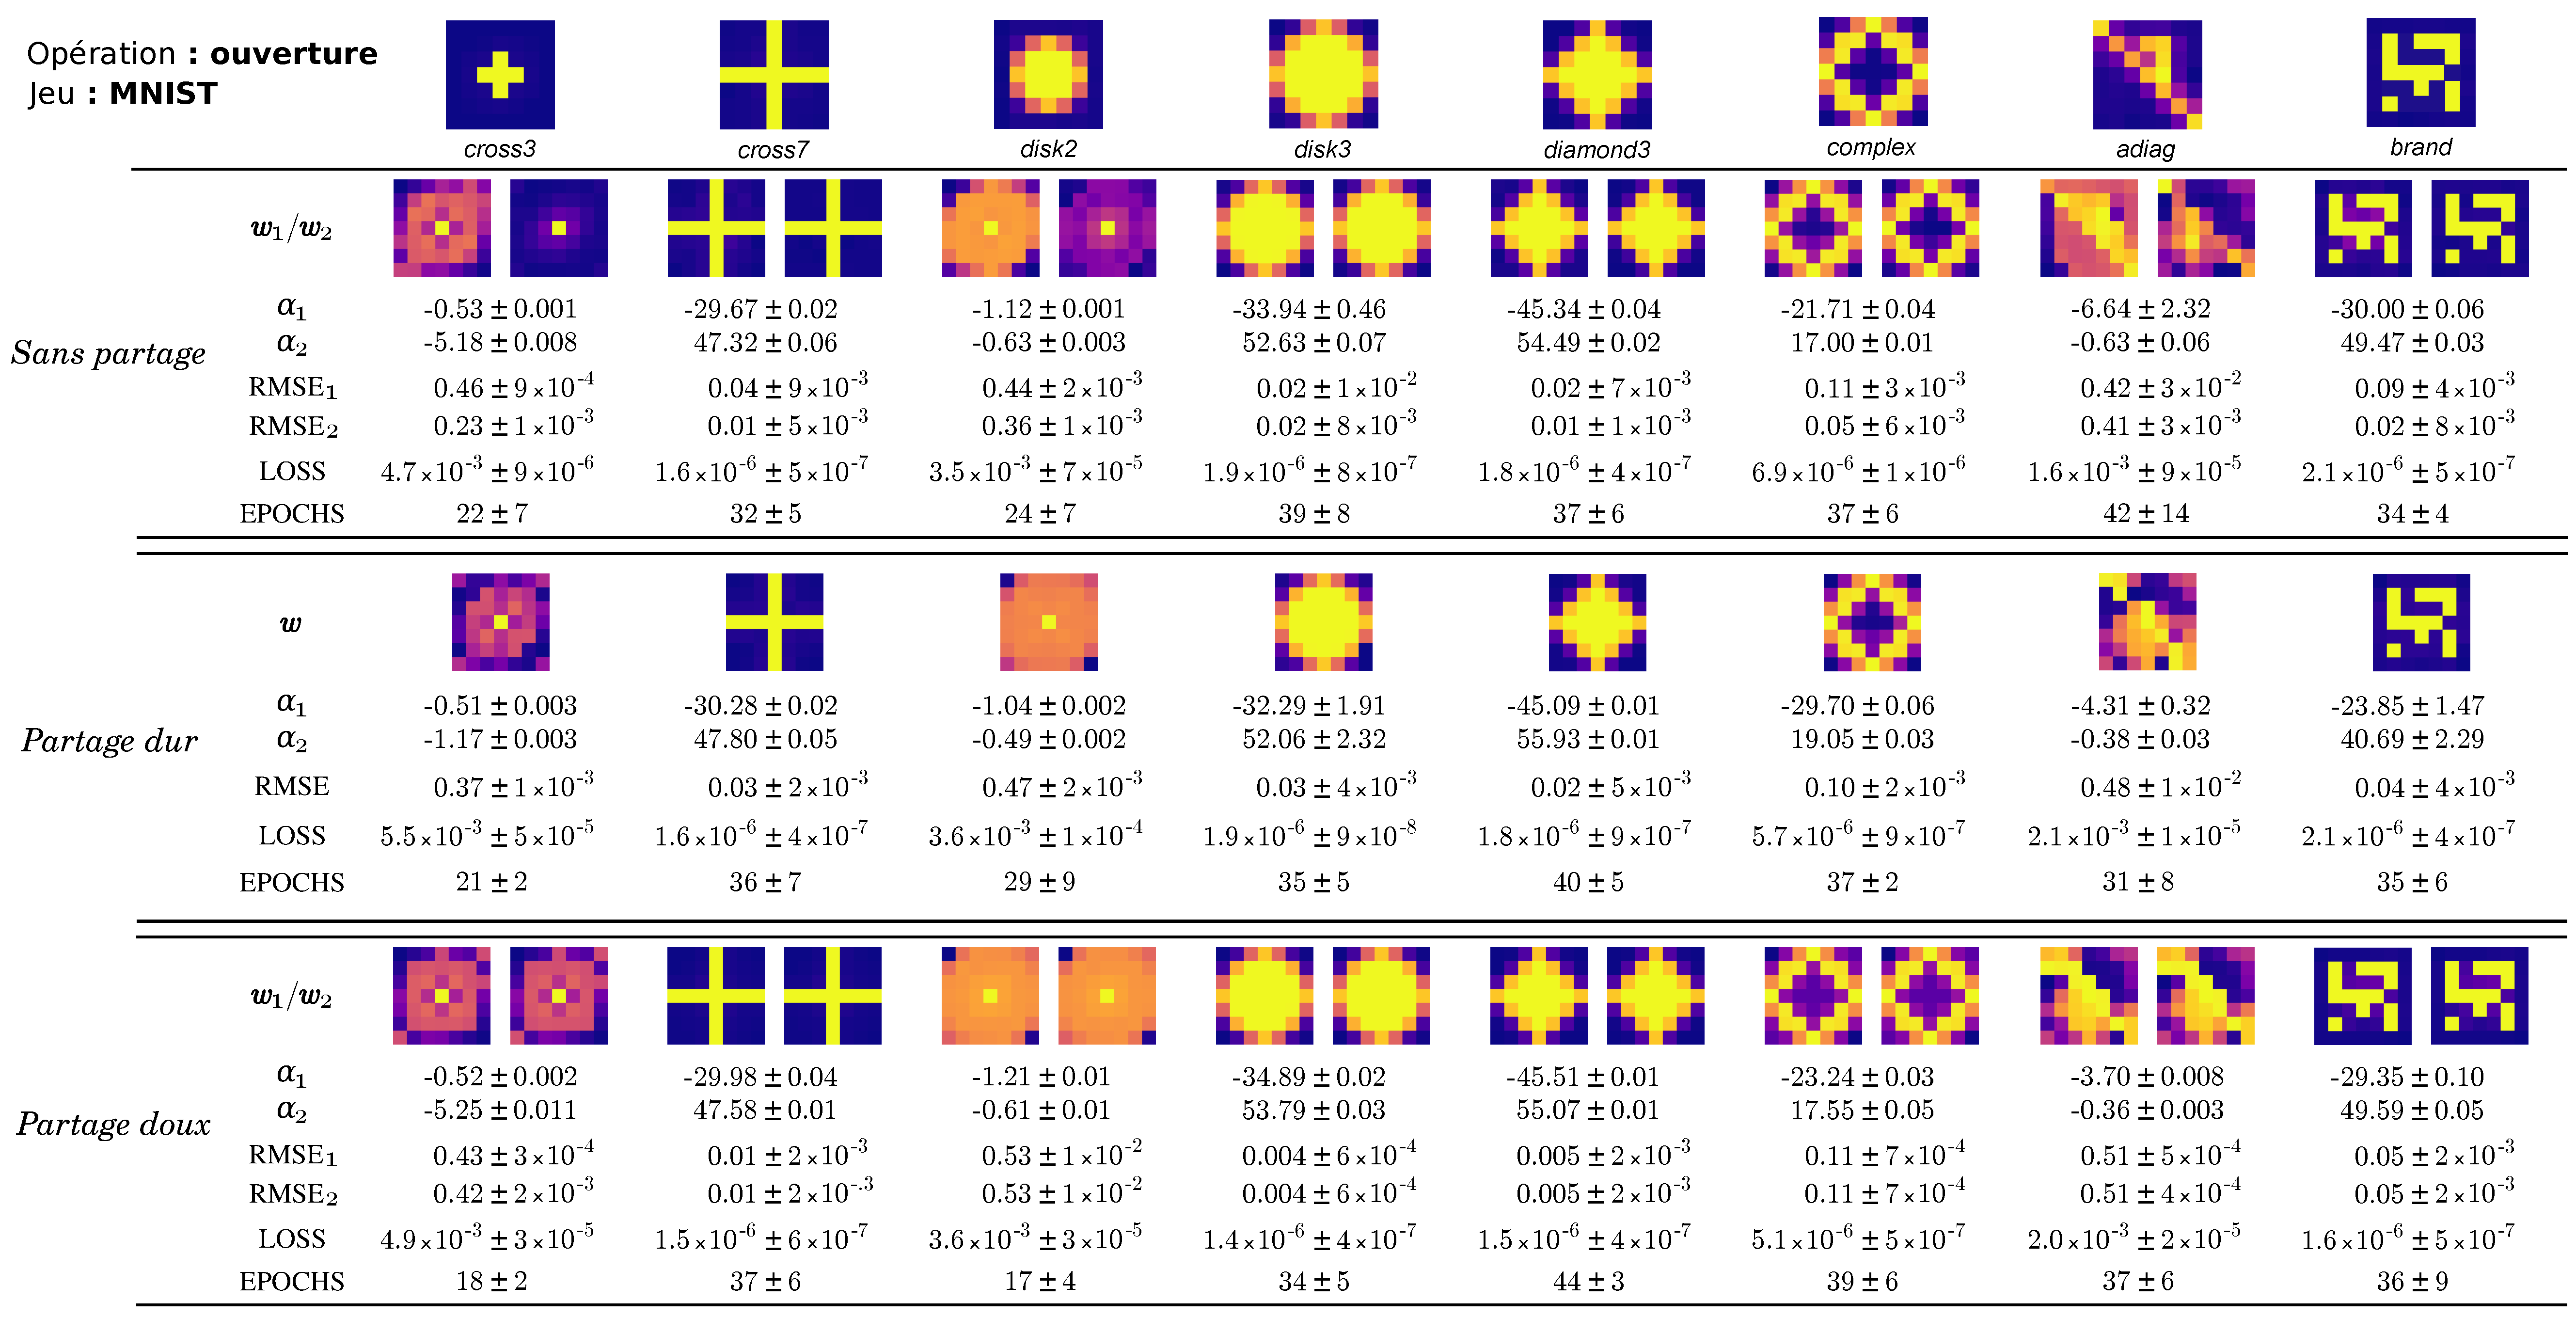
\includegraphics[width=1.00\linewidth]{parts/3-contributions/B-partage_de_poids/figures/h_opening_mnist.pdf}
    \vspace{-4.0mm}
    \caption{ \centering Comparaison des poids appris et des moyennes et écarts-types des métriques $\alpha$, \textit{RMSE}, \textit{loss} et nombre d'époques, et ce sur six runs, entre partage de poids dur, doux et sans partage, pour les huit fonctions structurantes cibles et l'opération d'\textbf{ouverture}.}
    \label{fig:MSEvsMSEpFSIM_opening}

    \bigskip

    \vspace{6.0mm}
    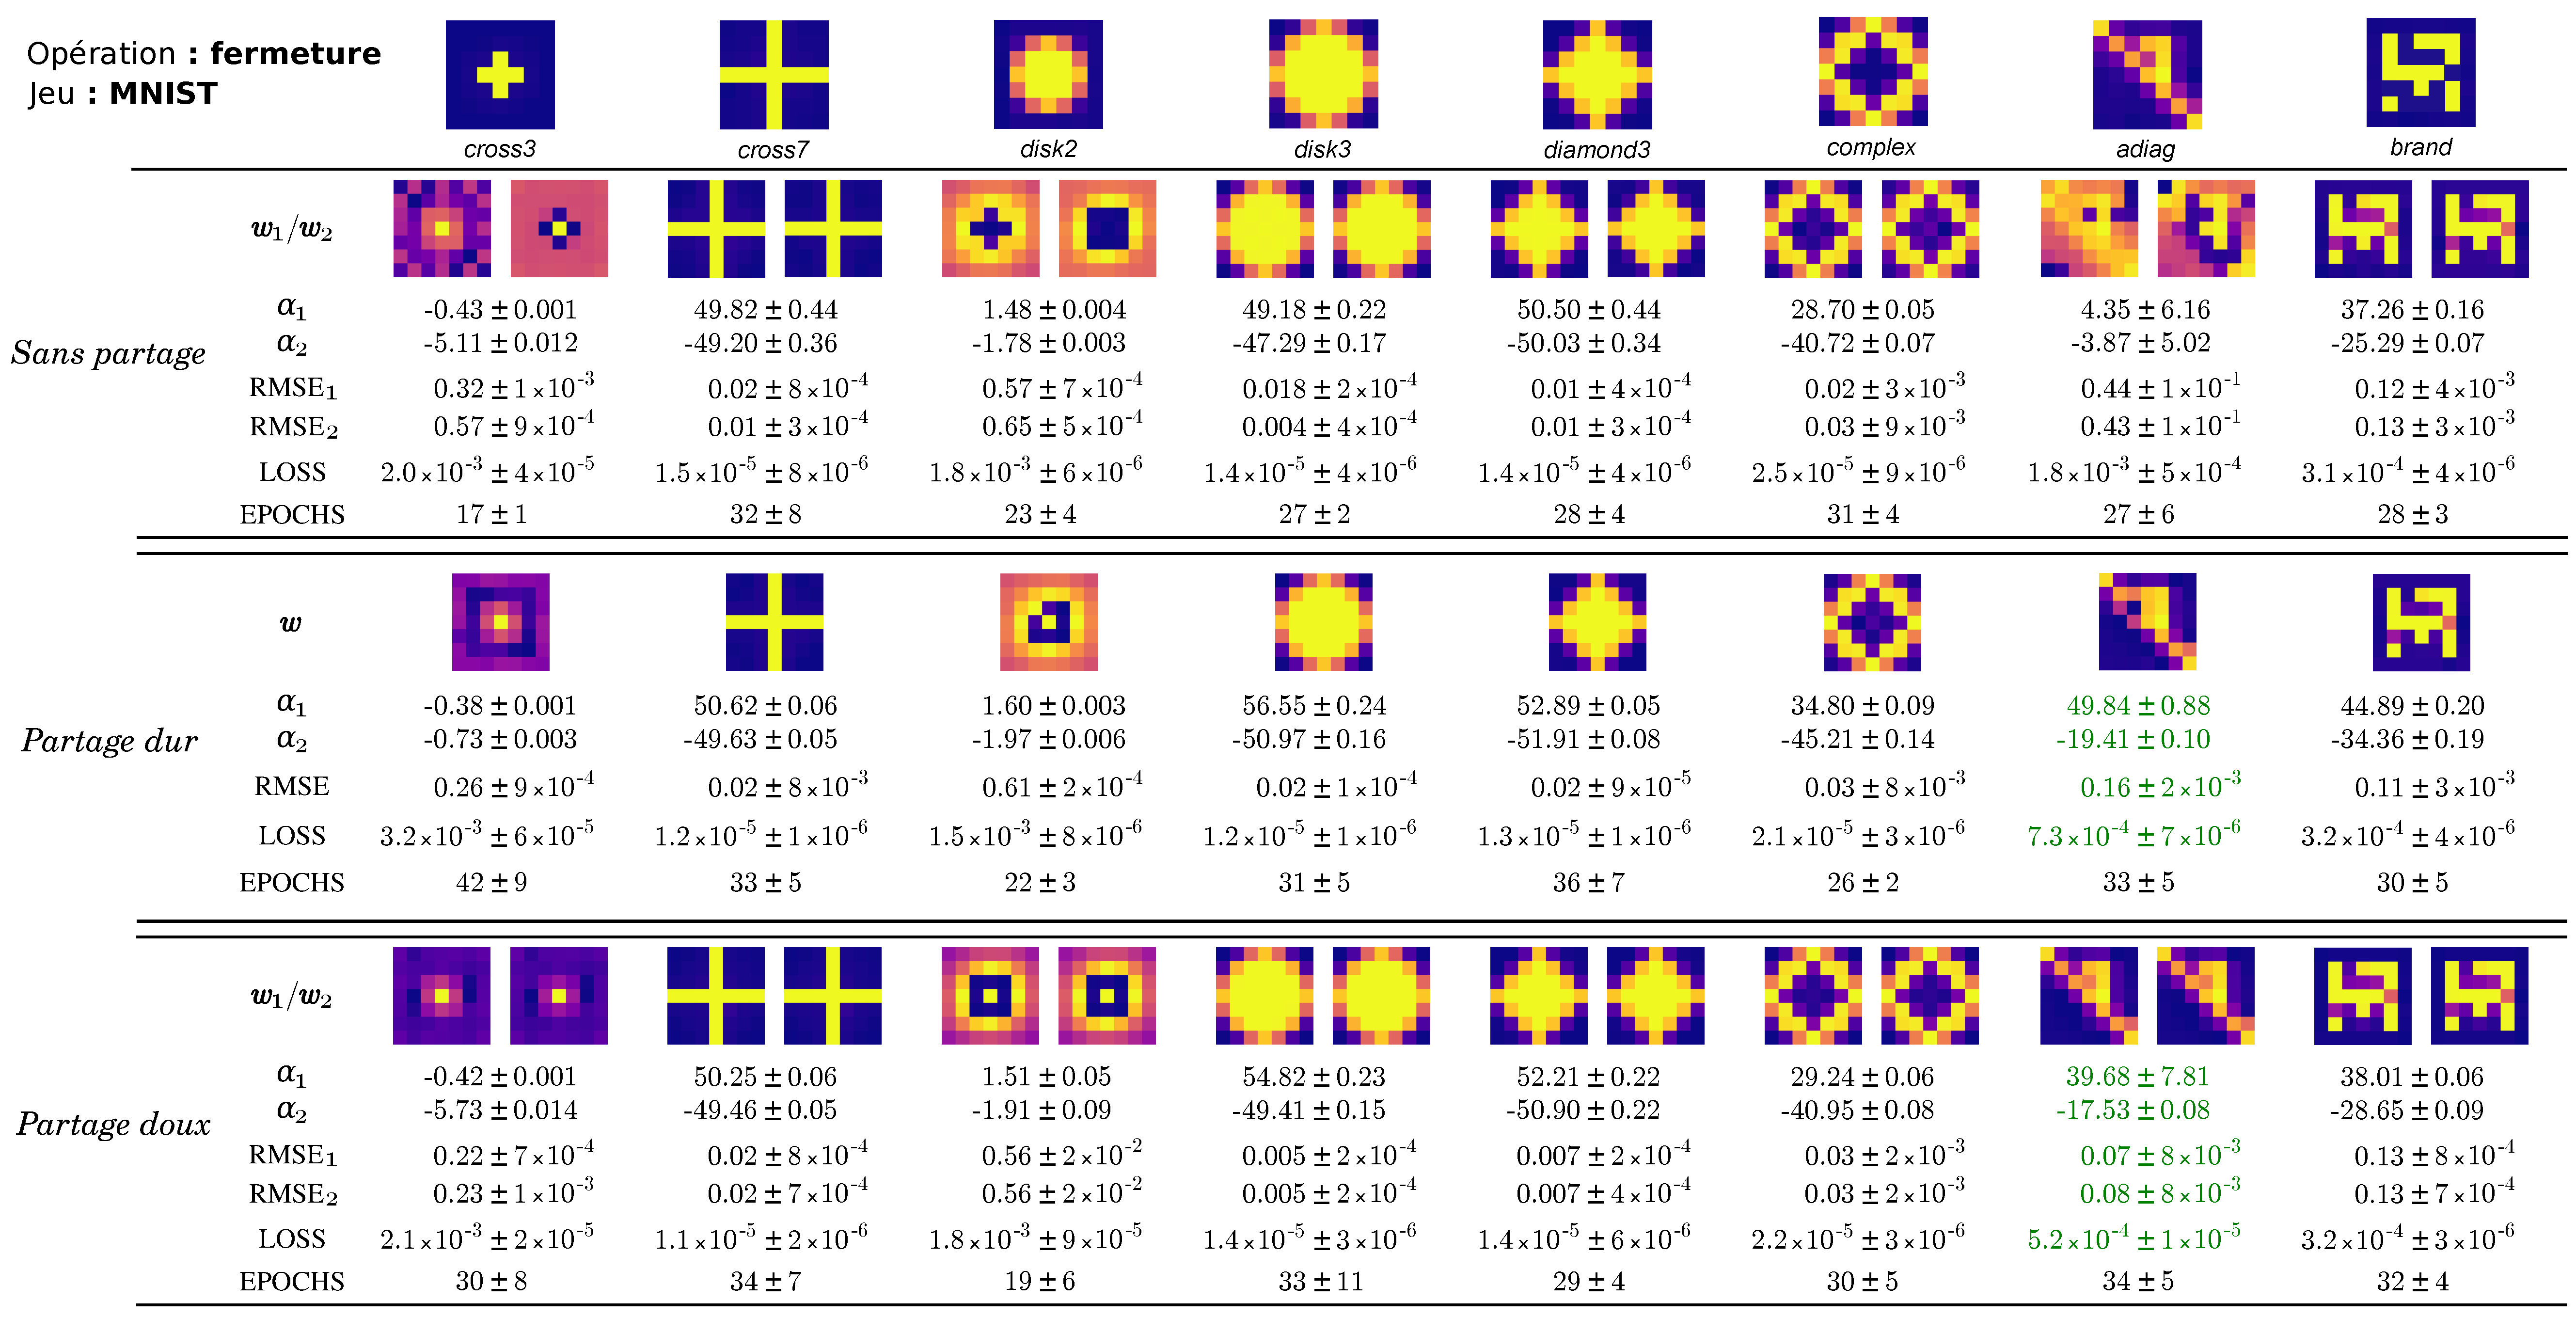
\includegraphics[width=1.00\linewidth]{parts/3-contributions/B-partage_de_poids/figures/h_closing_mnist.pdf}
    \vspace{-4.0mm}
    \caption{ \centering Comparaison des poids appris et des moyennes et écarts-types des métriques $\alpha$, \textit{RMSE}, \textit{loss} et nombre d'époques, et ce sur six runs, entre partage de poids dur, doux et sans partage, pour les huit fonctions structurantes cibles et l'opération de \textbf{fermeture}.}
    \label{fig:MSEvsMSEpFSIM_closing}
    
  \end{center}
\end{figure}


\newpage

%Les figures \ref{fig:MSEvsMSEpFSIM_opening} (ouverture) et \ref{fig:MSEvsMSEpFSIM_closing} (fermeture) montrent que les résultats de convergence des réseaux avec un partage des poids de leurs noyaux, que ce soit un partage dur ou doux, sont presque similaires aux résultats de ceux sans partage de poids. \\

%\vspace{-0.6mm}
Le réseau avec un partage de poids dur, comportant donc une couche duale, semble converger aussi bien voire un peu mieux que le réseau sans partage de poids. Dans les expériences où les réseaux sans partage de poids convergent initialement bien (\textit{cross7}, \textit{disk3}, \textit{diamond3}, \textit{complex} et \textit{brand}), ceux avec un partage de poids dur convergent au moins aussi bien, voire mieux dans certains cas (dans l'expérience avec la structure \textit{brand} et l'opération cible d'ouverture (fig. \ref{fig:MSEvsMSEpFSIM_opening}), il y a par exemple moins d'artéfacts sur le noyau de la couche duale que sur les noyaux du réseau sans partage). \\

\vspace{-3.0mm}
\noindent Dans les expériences où les réseaux sans partage de poids convergent, à l'inverse, initialement mal (forme des noyaux et valeurs des métriques trop mauvaises, comme \textit{cross3}, \textit{disk2} et \textit{adiag}), ceux avec un partage de poids dur convergent de la même manière, à l'exception de l'expérience avec la structure \textit{adiag} pour la fermeture (fig. \ref{fig:MSEvsMSEpFSIM_closing}), où le noyau de la couche converge ici vers la bonne forme cible, et où les métriques de performance du réseau présentent une perte \textit{loss} et une \textit{RMSE} bien plus faibles. \\

\vspace{-2.0mm}
Le réseau avec un partage doux, quant à lui, présente exactement les mêmes conclusions que le réseau avec un partage dur, bien que les formes des noyaux des réseaux et les métriques de performance soient légèrement différentes. Il présente des résultats similaires au réseau sans partage de poids. Comme pour le partage dur, seule l'expérience avec la structure \textit{adiag} pour l'opération de fermeture montre une bien meilleure convergence du réseau, avec une forme des noyaux proche de celle de la cible et de plutôt bons résultats au niveau des métriques de performance. \\

\vspace{-2.0mm}
En conclusion, ces deux méthodes de partage de poids des noyaux ne permettent pas forcément au réseau d'être plus efficace sur chaque expérience, mais résolvent tout de même le problème de convergence de \textit{adiag} pour la fermeture. De plus, elles donnent toutes deux des résultats similaires, bien que la forme des noyaux puisse être légèrement différente de l'un à l'autre sur certaines expériences. 
Les conclusions sont les mêmes avec la banque FashionMNIST, bien que les résultats soient assez différents. \\
%En conclusion, les réseaux implémentant ces deux méthodes de partage de poids peuvent être considérés comme équivalents aux réseaux sans partage, en terme d'efficacité et de précision. Ils ne sont donc pas forcément plus efficaces, mais résolvent tout de même le problème de convergence de \textit{adiag} pour la fermeture. De plus, les deux méthodes de partage de poids donnent des résultats similaires, bien que la forme des noyaux soient légèrement différents de l'un à l'autre sur certaines expériences. \\


%%%%%%%%%%%

%\vspace{1.6mm}
\noindent \textbf{Remarque :} \\

\vspace{-1.6mm}
\noindent Ici, on fait un partage de poids uniquement sur les noyaux. On aurait également pu partager inversement les $\alpha$ des deux couches, mais on considère qu'il s'agit là d'une bien trop forte hypothèse dans de nombreux contextes. En effet, pour des images cibles dont on ne connait pas l'ensemble des opérations duquel ces images résultent à partir d'images initiales, imposer au réseau bi-couches considéré de partir soit vers une opération de (pseudo-)ouverture soit vers une opération de (pseudo-)fermeture (car, dans un tel partage de poids, on imposerait une valeur opposée aux deux alphas du réseau) est une hypothèse déjà trop forte pour un tel système cible d'opérations inconnues, là où, au contraire, on peut se dire qu'il est plutôt plausible que les deux noyaux du réseau tendent à converger vers la même forme. Un tel partage inverse des $\alpha$ est cependant à considérer si l'on sait à l'avance que l'on veut soit un comportement d'ouverture soit de fermeture pour de tels réseaux à deux couches (partie suivante).
